\documentclass[11pt,a4paper]{article}
\usepackage[T1]{fontenc}
\usepackage[utf8]{inputenc}
\usepackage[magyar]{babel}
\usepackage{lmodern}
\usepackage{amsmath}
\usepackage{enumitem}
\usepackage{tikz}
\usepackage[a4paper,margin=2cm]{geometry}

\pagestyle{empty}
\setlength{\parindent}{0pt}

\begin{document}

\begin{enumerate}[leftmargin=*,label=\textbf{\arabic*.},itemsep=7pt,topsep=0pt,parsep=0pt]

\item Egy $m$ tömegű test $\alpha$ hajlásszögű lejtőn csúszik lefelé; a csúszási
súrlódási együttható $\mu$.
\textbf{a)} Írd fel a test gyorsulását $m$, $\alpha$, $\mu$ és $g$ segítségével --
számok nélkül
\textbf{b)} Milyen $\alpha$ hajlásszög esetén nem indul el a nyugvó test?
\textbf{c)} Mi változik, ha a testet felfelé lökjük meg a lejtőn?
\textbf{d)} Ellenőrizd a kapott összefüggést a $\mu\to 0$, az $\alpha\to 0$ és az
$\alpha\to 90^\circ$ határesetben!

\item
\begin{minipage}[t]{0.55\linewidth}
Az ábrán egy egyenes vonalú mozgás $v$--$t$ grafikonja látható.
\textbf{a)} Mekkora a test által megtett teljes út?
\textbf{b)} Rajzold fel ugyanennek a mozgásnak az $a$--$t$ grafikonját!
\end{minipage}\hfill
\begin{minipage}[t]{0.42\linewidth}
\vspace{0pt}
\centering
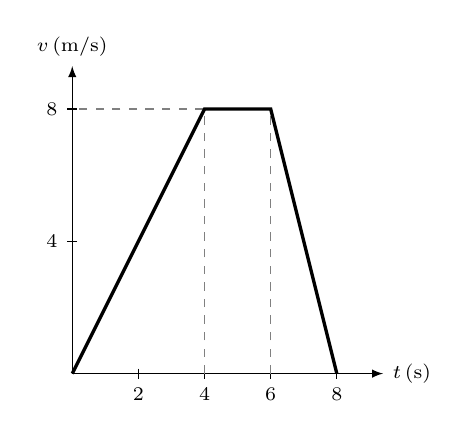
\begin{tikzpicture}[scale=0.42,>=latex]
  \draw[->] (0,0) -- (9.4,0) node[right] {\scriptsize $t$\,(s)};
  \draw[->] (0,0) -- (0,9.3) node[above] {\scriptsize $v$\,(m/s)};
  \foreach \x in {2,4,6,8} \draw (\x,0.15) -- (\x,-0.15) node[below] {\scriptsize \x};
  \foreach \y in {4,8} \draw (0.15,\y) -- (-0.15,\y) node[left] {\scriptsize \y};
  \draw[gray,dashed] (4,0) -- (4,8) -- (0,8);
  \draw[gray,dashed] (6,0) -- (6,8);
  \draw[very thick] (0,0) -- (4,8) -- (6,8) -- (8,0);
\end{tikzpicture}
\end{minipage}

\item Egy testet 20~m magasról ejtünk el kezdősebesség nélkül (a közegellenállástól
eltekintünk). Mekkora a becsapódási sebessége? Oldd meg a feladatot kétféleképpen:
kinematikai úton és az energiamegmaradás tételével!

\item Egy könyv nyugalomban fekszik a vízszintes asztallapon. Sorold fel a fellépő
erőket, és párosítsd őket Newton III.\ törvénye (a hatás--ellenhatás törvénye)
szerint! Melyik erő melyiknek az ellenereje?

\item
\begin{minipage}[t]{0.55\linewidth}
Egy ideális gáz az ábrán látható körfolyamatot végzi: izoterm tágulás
($A\!\to\!B$), izochor melegítés ($B\!\to\!C$), majd izobár összenyomás
($C\!\to\!A$). Add meg minden szakaszra a gáz által végzett munka és a gáz által
felvett hő előjelét, és indokold meg a válaszodat!
\end{minipage}\hfill
\begin{minipage}[t]{0.42\linewidth}
\vspace{0pt}
\centering
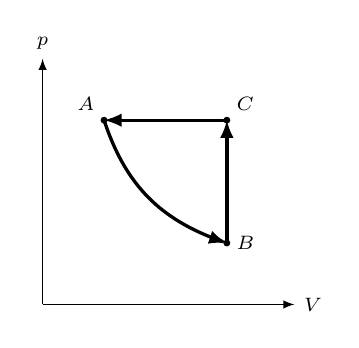
\begin{tikzpicture}[scale=0.78,>=latex]
  \draw[->] (0,0) -- (4.1,0) node[right] {\scriptsize $V$};
  \draw[->] (0,0) -- (0,4.0) node[above] {\scriptsize $p$};
  \draw[very thick,->,domain=1:3,smooth,variable=\x] plot ({\x},{3/\x});
  \draw[very thick,->] (3,1) -- (3,3);
  \draw[very thick,->] (3,3) -- (1,3);
  \fill (1,3) circle (1.6pt) node[above left] {\scriptsize $A$};
  \fill (3,1) circle (1.6pt) node[right] {\scriptsize $B$};
  \fill (3,3) circle (1.6pt) node[above right] {\scriptsize $C$};
\end{tikzpicture}
\end{minipage}

\item Egy rúdmágnest az északi pólusával közelítünk egy rézgyűrű felé. Milyen
irányú áram indukálódik a gyűrűben, és milyen irányú erő hat a mágnesre? Indokold
a válaszodat a Lenz-törvénnyel!

\item Rendelkezésedre áll egy mérőszalag és egy stopper. Tervezz mérést a
nehézségi gyorsulás meghatározására! Írd le a mérés menetét, és add meg, hogy
melyik mennyiség mérési hibája okozza a legnagyobb bizonytalanságot az
eredményben!

\end{enumerate}

\end{document}
